% !TEX root = ../main.tex
%
% ========
\chapter{Particle interferometry}
\label{ch:pi}
% ========
  Two-particle interferometry (also called \textit{femtoscopy}) gives a possibility to investigate space-time characteristics of the particle-emitting source created in heavy ion collisions.
  Through the study of particle correlations, their momentum distributions can be used to obtain information about the spatial extent of the created system.
  Using this method, one can measure sizes of the order of $10^{-15}$ m and times of the order of $10^{-23}$ s.
  %
  % ========
  \section{The HBT interferometry}
  % ========
    In 1956, Robert Hanbury Brown and Richard Q. Twiss proposed a method which allowed to investigate angular dimensions of stars through analysis of interference between photons.
    They performed a measurement of the intensity of a beam of light coming from a star using two detectors separated in space.
    In a signal plotted as a function of distance between detectors an interference effect was observed. Despite the fact that no phase information was collected, a positive correlation was visible.
    Hanbury Brown and Twiss used this interference signal to calculate the angular size of a star with excellent resolution.
    In principle, the HBT interferometry was designed for astronomy purposes, however it can be also used to measure extent of any emitting source.
    Therefore, it was adapted to heavy ion collisions to investigate dimensions of a particle-emitting source~\cite{drkisiel}.
  %
  % ========
  \section{Theoretical approach}
  % ========
    Intensity interferometry in heavy ion physics uses similar mathematical formalism as the astronomy HBT measurement.
    The difference between them is that femtoscopy uses a two-particle relative momentum and yields the space-time picture of a source, whereas the latter method uses the distance between detectors to calculate angular size of the star.
    %
    % ========
    \subsection{Conventions used}
    % ========
      In heavy ion collisions to describe particular directions, components of momentum and location of particles, one uses naming convention called the Bertsch-Pratt coordinate system.
      This system is presented in Fig.~\ref{fig:coordinate-system}.
      \begin{figure}[h]
        \centering
        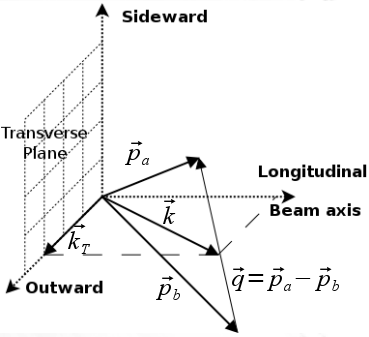
\includegraphics[width=0.5\textwidth]{coordinate_system}
        \caption{Bertsch-Pratt directions naming convention used in heavy ion collision.}
        \label{fig:coordinate-system}
      \end{figure}
      The three directions are called \textit{longitudinal}, \textit{outward} and \textit{sideward}.
      The longitudinal direction is parallel to the beam axis.
      The plane perpendicular to the beam axis is called a \textit{transverse plane}.
      A projection of a particle pair momentum $\vect{k} = (\vect{p}_a + \vect{p}_b)/2$ on a transverse plane (a \textit{transverse momentum} $\vect{k}_T$) determines the \textit{outward} direction: $(\vect{k})_{out} = \vect{k}_T$.
      A direction which is perpendicular to the longitudinal and outward ones is called \textit{sideward}.

      A particle pair is usually described using two coordinate systems.
      The first one, \textit{Longitudinally Co-Moving System} (\textbf{LCMS}) is moving along the particle pair with the longitudinal direction in the other words, the pair longitudinal momentum vanishes: $(\vect{p}_a)_{long} = -(\vect{p}_b)_{long} $.
      The second system is called \textit{Pair Rest Frame} (\textbf{PRF}).
      In the PRF the centre of mass rests: $\vect{p}_a = -\vect{p}_b$.
      Variables which are expressed in the PRF are marked with a star (e.g. $\vect{k}^{*}$).

      The transition of space-time coordinates from LCMS to PRF is simply a boost along the outward direction, with the transverse velocity of the pair~$\beta_T = (\vect{v}/c)_{out}$~\cite{nonidfemto}:
      \begin{align}
        \label{eq:lcmstoprf}
        r^{*}_{out} &= \gamma_{t}(r_{out} - \beta_T \Delta t)~,\\
        r^{*}_{side} &= r_{side}~,\\
        r^{*}_{long} &= r_{long}~,\\
        \Delta t^{*} &= \gamma_T(\Delta t - \beta_T r_{out})~, 
      \end{align}
      where $\gamma_T = (1-\beta^{2}_T)^{-1/2}$ is the Lorentz factor.
      However, in calculations performed in this work the equal time approximation is used which assumes that particles in a pair were produced at the same time in PRF - the $\Delta t^{*}$ is neglected.

      The most important variables used to describe particle pair are total momentum $\vect{P} = \vect{p}_a + \vect{p}_b$ and relative momentum $\vect{q} = \vect{p_a} - \vect{p_b}$.
      In PRF, the following relation $\vect{q} = 2 \vect{k}^{*}$ is also valid, where $\vect{k}^{*}$ is a momentum of the first particle in PRF.

    %
    % ========
    \subsection{Two particle wave function}
    % ========
      Let us consider two identical particles with momenta $\vect{p_1}$ and $\vect{p_2}$ emitted from space points $\vect{x_1}$ and $\vect{x_2}$.
      These particles can be treated as two incoherent waves.
      \begin{figure}[h]
        \centering
        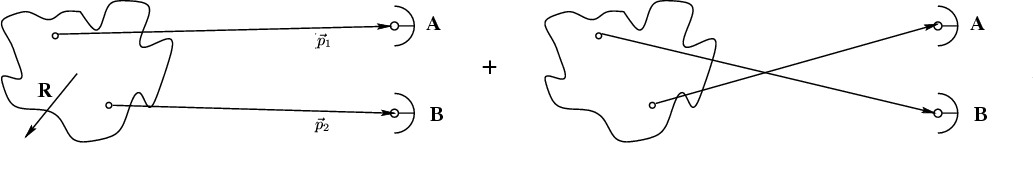
\includegraphics[width=0.9\textwidth]{wavefunction}
        \caption{The pair wave function is a superposition of all possible states. In case of particle interferometry it includes two cases: particles with momenta $p_1$,~$p_2$ registered by detectors \textit{A}, \textit{B} and $p_1$,~$p_2$ registered by \textit{B}, \textit{A} respectively.}
        \label{fig:wavefunction}
      \end{figure}
      If the particles are identical, they are also indistinguishable.
      Therefore, one has also take into account the scenario, where the particle with momentum $\vect{p_1}$ is emitted from $\vect{x_2}$ and particle $\vect{p_2}$ from $\vect{x_1}$ (Fig.~\ref{fig:wavefunction}).
      In such case, the wave function describing behaviour of a pair has to contain both components~\cite{drkisiel}:
      \begin{equation}
      \label{eq:wavefunction}
        \Psi_{ab}(\vect{q})=\frac{1}{\sqrt{2}} \left[ \exp(- i \vect{p_1}\vect{x_1} - i \vect{p_2}\vect{x_2}) \pm \exp(- i \vect{p_2}\vect{x_1} - i \vect{p_1}\vect{x_2}) \right]~.
      \end{equation}
      While in the case of identical bosons it is symmetric (``+'' sign in Eq.~\ref{eq:wavefunction}) and in case of identical fermions - antisymmetric (``-'' sign).
      This anti-symmetrization or symmetrization implies the correlation effect coming from the Fermi-Dirac or Bose-Einstein statistics accordingly.
      The exact wave function forms used in calculations in this work are given by:
      \begin{align}
        \label{eq:pipi-wf}
        |\Psi_{\pi\pi}(\vect{r^*},\vect{k^*})|^2 = |\Psi_{KK}(\vect{r^*},\vect{k^*})|^2 &= 1 + \cos(2 \vect{k^*} \vect{r^*})~, \\
        \label{eq:pp-wf}
        |\Psi_{pp}(\vect{r^*},\vect{k^*})|^2 &= 1 - \frac{1}{2} \cos(2 \vect{k^*} \vect{r^*})~.
      \end{align}
      The first one is used in the case of identical bosons, and the latter one is for identical fermions.
      A wave function for pair of spin-1/2 fermions (Eq.~\ref{eq:pp-wf}) is a superposition of two possible states: singlet state (with spin equal to 0 and one eigenstate) and triplet state (with spin equal to 1 and three possible eigenstates).
      For the singlet state, a wave function is symmetric and for the triplet state, it is antisymmetric.
      In other words, the $|\Psi_{pp}|^2$ encodes correlation coming from Bose-Einstein statistics (with weight $1/4$) and anti-correlation from Fermi-Dirac distribution (with weight $3/4$).

      In femtoscopy one usually performs full analysis of a correlation function through the comparison to its analytical form.
      In this case, the pair wave function has to include all kinds of interactions between particles.
      However, the aim of this work is an analysis of femtoscopic radii proportional to the inverse of a width of a correlation function (for detailed description see Section~\ref{sec:correlation-function}).
      This width is determined by effects coming from quantum statistics.
      Besides, the influence of other effects (like Final State Interactions) on femtoscopic radius is small.
      Moreover, the inclusion of Final State Interactions in computation increase its complexity and required time.
      Hence, one can calculate the correlation function using only the quantum statistics and still be able to extract femtoscopic information.

    %
    % ========
    \subsection{Source emission function}
    \label{sec:source-emission-function}
    % ========
      To describe a particle emitting source, one uses a single-particle emission function~\cite{nonidfemto}:
      \begin{equation}
        \label{eq:source-single-3d}
        S_A(\vect{x}_1,\vect{p}_1) = \int S(\vect{x}_1,\vect{p}_1,\vect{x}_2,\vect{p}_2,...,\vect{x}_N,\vect{p}_N)
        d \vect{x}_2 d \vect{p}_2 ... d \vect{x}_N d \vect{p}_N
      \end{equation}
      and a two-particle one:
      \begin{equation}
        \label{eq:source-two-3d}
        S_{AB}(\vect{x}_1,\vect{p}_1,\vect{x}_2,\vect{p}_2) = \int S(\vect{x}_1,\vect{p}_1,\vect{x}_2,\vect{p}_2,...,\vect{x}_N,\vect{p}_N)
        d \vect{x}_3 d \vect{p}_3 ... d \vect{x}_N d \vect{p}_N~.
      \end{equation}
      Emission function $S(\cdot)$ can be interpreted as a probability to emit a particle, or a pair of particles from a given space-time point with a certain momentum.
      In principle, the source function should encode all physics aspects of the particle generation process i.e. the symmetrization for bosons and fermions, as well as the two-body and many body Final State Interactions.
      Instead of this, one usually assumes that each particle's emission process is independent - the interaction between final-state particles after their creation is not related with their generation process.
      This assumption allows to construct two-particle emission function from single particle emission functions via a convolution~\cite{nonidfemto}:
      \begin{equation}
        \label{eq:source-two-conv}
        \begin{split}
          S(\vect{k}^{*},\vect{r}^{*}) = \int S_A ( \vect{p}_1, \vect{x}_1 ) S_B ( \vect{p}_2, \vect{x}_2 )
          \delta \left[\vect{k}^{*} - \frac{\vect{p}_1+\vect{p}_2}{2} \right]
          \delta \left[\vect{r}^{*} - (\vect{x}_1-\vect{x}_2) \right] \\
          \times~d^4 \vect{x}_1 d^4 \vect{x}_2 d^4 \vect{x}_1 d^3 \vect{p}_1 d^3 \vect{p}_2~.
        \end{split}
      \end{equation}
      In principle, Eq.~\ref{eq:source-two-conv} is not reversible - an information about $S_A(\cdot)$ cannot be derived from $S_{AB}(\cdot)$.
      In the case of identical particles ($S_A = S_B$), one can make further simplifications.
      Femtoscopy can give information only about two-particle emission function.
      Moreover, convolution of the two identical Gaussian distributions is also a Gaussian distribution with $\sigma$ multiplied by $\sqrt{2}$.
      Hence, when considering Gaussian distribution as a source function in Eq.~\ref{eq:source-two-conv}, one can obtain a $\sigma$ of a single emission function from a two-particle one.
      % An exception from this rule is a Gaussian source function, hence it is often used in femtoscopic calculations.
      Considering pairs of identical particles, an emission function is assumed to be described by the following equation in Pair Rest Frame~\cite{nonidfemto}:
      \begin{equation}
        S^{PRF}_{1D} (\vect{r}^{*}) = \exp \left( - \frac{ {r_{out}^*}^{2} + {r_{side}^*}^{2} + {r_{long}^*}^{2}}{4 {R_{inv}}^2} \right)~.
      \end{equation}
      To make a transition from the three-dimensional variables to the one-dimensional variables, the proper Jacobian is required~${r^*}^2$:
      \begin{empheq}[innerbox=\fbox, right=~.]{align}
        \label{eq:source-1d-prf}
        S^{PRF}_{1D} (r^{*}) = {r^*}^{2} \exp \left( - \frac{{r^*}^{2}}{4 {R_{inv}}^2} \right)
      \end{empheq}
      The ``4'' in the denominator before the $R_{inv}$ in Eq.~\ref{eq:source-1d-prf} comes from the convolution of the two Gaussian distributions, which multiplies the $R_{inv}$ by a factor of $\sqrt{2}$.

      The emission function in a more complex form was used by all RHIC and SPS experiments in identical pion femtoscopy:
      \begin{empheq}[innerbox=\fbox, right=~.]{align}
        \label{eq:source-3d-lcms}
        S^{LCMS}_{3D} (\vect{r}) = \exp \left( 
          - \frac{ r_{out}^{2}}{4 {R_{out}}^2}
          - \frac{ r_{side}^{2}}{4 {R_{side}}^2}
          - \frac{ r_{long}^{2}}{4 {R_{long}}^2}
        \right)
      \end{empheq}
      The main difference is that it contains three different and independent widths $R_{out}$, $R_{side}$, $R_{long}$ and they are defined not in PRF, but in LCMS.
      Unlike in PRF, in LCMS an equal-time approximation is not used.
      For identical particles this is not a problem - only Coulomb interaction inside a wave function depends on $\Delta t$.
      %
      % ========
      \subsubsection{Relationship between one-dimensional and three-dimensional source sizes}
      % ========
      Up to now, most of femtoscopic measurements were limited only to averaged source size $R^L_{av}$ (the letter ``L'' in superscript stands for LCMS):
      \begin{equation}
        S^{LCMS}_{1D} (\vect{r}) = \exp \left( - \frac{ {r_{out}}^{2} + {r_{side}}^{2} + {r_{long}}^{2}}{2 {R^{L}_{av}}^2} \right)~.
      \end{equation}
      The relationship between $S^{LCMS}_{1D}(\cdot)$ and $S^{LCMS}_{3D}(\cdot)$ is given by:
      \begin{equation}
        \begin{split}
        \label{eq:source-1d-from-3d}
        S^{LCMS}_{3D} (r) = \int \exp \left( 
          - \frac{ r_{out}^{2}}{2 {R^L_{out}}^2}
          - \frac{ r_{side}^{2}}{2 {R^L_{side}}^2}
          - \frac{ r_{long}^{2}}{2 {R^L_{long}}^2}
        \right)
        \\ \times~\delta \left(
          r - \sqrt{ r_{out}^{2} + r_{side}^{2} + r_{long}^{2}}
        ~\right)
        d r_{out} d r_{side} d r _{long}~.
        \end{split}
      \end{equation}
      The one-dimensional source size corresponding to the three-dimensional one can be approximated by the following form:
      \begin{equation}
        \label{eq:source-1d-lcms}
        S^{LCMS}_{1D} (r) = {r}^{2} \exp \left( - \frac{r^{2}}{2 {R^L_{av}}^2} \right)~.
      \end{equation}
      The above equation assumes that $R^L_{out} = R^L_{side} = R^L_{long}$ hence $R^L_{av} = R^L_{out}$.
      \begin{figure}[b]
        \centering
        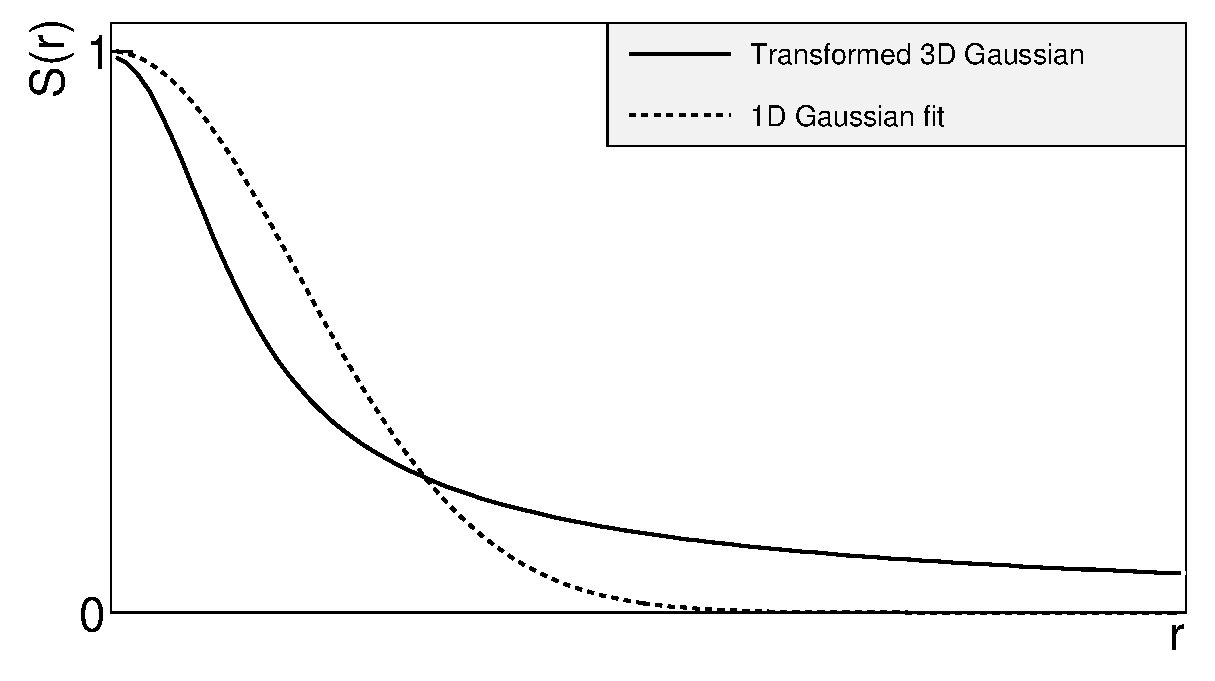
\includegraphics[width=0.7\textwidth]{3dg21d}
        \caption{A three-dimensional Gaussian source function with different widths was transformed into one-dimensional function. To illustrate deformations, one-dimensional Gaussian distribution was fitted.}
        \label{fig:3dgaussian}
      \end{figure}
      If the last condition is not satisfied, one can not give an explicit mathematical relation between one-dimensional and three-dimensional source sizes.
      However, for realistic values of $R$ (i.e. for similar values of $R_{out}$, $R_{side}$, $R_{long}$), the $S^{LCMS}_{3D}$ from Eq.~\ref{eq:source-1d-from-3d} is not very different from Gaussian distribution and can be well approximated by Eq.~\ref{eq:source-1d-lcms}.

      A deformation of an averaged source function caused by big differences between $R_{out}$, $R_{side}$, $R_{long}$ is presented in the Fig.~\ref{fig:3dgaussian}.
      A three-dimensional Gaussian distribution with varying widths was projected into one-dimensional function using the Eq.~\ref{eq:source-1d-from-3d}.
      Afterwards, an one-dimensional Gaussian distribution was fitted.
      One can notice a heavy tail of an averaged distribution in the large $r$ region, which makes this approximation using one-dimensional distribution in this case quite inaccurate.
      
      One can obtain a relation between one-dimensional width and three-dimensional ones from Eq.~\ref{eq:source-1d-from-3d} and Eq.~\ref{eq:source-1d-lcms} through numerical calculations~\cite{nonidfemto}:
      \begin{empheq}[innerbox=\fbox, right=~.]{align}
        \label{eq:3dradiito1d}
        R^{L}_{av} = \sqrt{ \left. \left( {R^L_{out}}^2 + {R^L_{side}}^2 + {R^L_{long}}^2 \right) \middle/ 3 \right. }
      \end{empheq}
      This equation does not depend on the pair velocity, hence it is valid both in LCMS and PRF.
    %
    % ========
    \FloatBarrier
    \subsection{Analytical form of a correlation function}
    \label{sec:correlation-function}
    % ========
      The fundamental object in a particle interferometry is a correlation function defined as:
      \begin{equation}
        \label{eq:th_cf}
        C(\vect{p}_a,\vect{p}_b) = \frac{P_2(\vect{p}_a,\vect{p}_b)}{P_1(\vect{p}_a) P_1(\vect{p}_b)}~,
      \end{equation}
      where $P_2$ is a conditional probability to observe a particle with momentum $\vect{p}_b$ if particle with momentum $\vect{p}_a$ was also observed, while a $P_1$ is a probability to register a particle with a given momentum.
      The relationship between source emission function, pair wave function and the correlation function is described by the following equation:
      \begin{equation}
        \label{eq:cf_integral}
        C(\vect{p}_1,\vect{p}_2) = \int S_{AB}(\vect{p}_1,\vect{x}_1,\vect{p}_2,\vect{x}_2)
          |\Psi_{AB}|^2 d^4 \vect{x}_1 d^4 \vect{x}_2~.
      \end{equation}
      Substituting the one-dimensional emission function (Eq.~\ref{eq:source-1d-prf}) into the above equation leads to the following form of correlation function in PRF:
      \begin{empheq}[innerbox=\fbox, right={~,}]{align}
        \label{eq:cf_1d}
        C(q) = 1 + \lambda \exp \left( - R_{inv}^2 q^2 \right)
      \end{empheq}
      where $q$ is a momentum difference between two particles.
      On the other hand, using the three-dimensional emission function (Eq.~\ref{eq:source-3d-lcms}) one gets the following correlation function defined in LCMS:
      \begin{empheq}[innerbox=\fbox, right={~,}]{align}
        \label{eq:cf_3d}
        C(\vect{q}) = 1+ \lambda \exp \left( -R_{out}^2 q_{out}^2 -R_{side}^2 q_{side}^2 -R_{long}^2 q_{long}^2  \right)
      \end{empheq}
      where $q_{out}$, $q_{side}$, $q_{long}$ are $\vect{q}$ components in the outward, sideward and longitudinal directions.
      The $\lambda$ parameter in the above equations determines the correlation strength.
      In principle, the $\lambda$ coefficient has values in the range $\lambda \in [-0.5,1]$ which depends on the pair type.
      In the case of pairs of identical bosons (like $\pi$-$\pi$ or $K$-$K$) the $\lambda \to 1$ while for identical fermions (e.g. $p$-$p$) $\lambda \to$~-0.5.
      Values of $\lambda$ observed experimentally are lower than 1 (for bosons) and greater than -0.5 (for fermions).
      There are few explanations to this effect: detector's efficiencies, inclusion of misidentified particles in a used sample or inclusion of non-correlated pairs (when one or both particles come from e.g. long-lived resonance).
      The analysis carried out in this work uses data from a model, therefore the detector efficiency and particle's purity is not taken into account~\cite{nonidfemto}.
    %
    % ========
    \subsection{Spherical harmonics decomposition of a correlation function}
    \label{sec:sh}
    % ========
      The results coming from an analysis using three-dimensional correlation function in Cartesian coordinates are quite difficult to visualize.
      To do that, one usually performs a projection into one dimension in outward, sideward and longitudinal directions. 
      However, important information about a correlation function may be lost in this procedure, because it gives only a limited view of the full three-dimensional structure.
      Recently, a more advanced way of presenting correlation function - a spherical harmonics decomposition, was proposed.
      In this method, the three-dimensional correlation function is decomposed into an infinite set of components in a form of one-dimensional histograms $C^m_l (q)$.
      In this representation, a correlation function is defined as a sum of a series~\cite{sh}:
      \begin{equation}
        C(\vect{q}) = \sum_{l,m} C^m_l (q) Y^m_l(\theta, \phi)~.
      \end{equation}
      Spherical harmonics $Y^m_l(\theta,\phi)$ are an orthogonal set of solutions to the Laplace's equation in spherical coordinates.
      Hence, in this approach, a correlation function is defined as a function of $q$, $\theta$ and $\phi$.
      To obtain $C^m_l$ coefficients in the series, one has to calculate the following integral:
      \begin{equation}
        \label{eq:sh_decomposition}
        C^m_l(q) = \int_\Omega C(q,\theta,\phi) Y^{m*}_l (\theta,\phi) d \Omega~,
      \end{equation}
      where $\Omega$ is a full solid angle.

      Spherical harmonics representation has several important advantages.
      First of all, it requires less statistics than traditional analysis performed in Cartesian coordinates.
      Moreover, it encodes full three-dimensional information in a set of one-dimensional plots. 
      However, the full description of a correlation function requires infinite number of \textit{l} and \textit{m} components.
      But it so happens that the intrinsic symmetries of a pair distribution in a femtoscopic analysis result in a fact that most of the components vanish.
      For the identical particles correlation function, all coefficients with odd values of \textit{l} and \textit{m} disappear.
      % Because the values of a correlation function are real, the imaginary part of a series are equal to zero ($\Im C^m_l = 0$).
      It has been also shown that the most significant portion of femtoscopic data is stored in the components with the lowest \textit{l} values.
      It is expected that the main femtoscopic information is contained in the following components~\cite{nonidfemto}:
      \begin{align}
        C^0_0 &\to R_{LCMS}~, \\
        \Re C^0_2 &\to \frac{R_T}{R_{long}}~, \\
        \Re C^2_2 &\to \frac{R_{out}}{R_{side}}~,
      \end{align}
      where $R_{LCMS} = \sqrt{ \left. \left( {R_{out}}^2 + {R_{side}}^2 + {R_{long}}^2 \right) \middle/ 3 \right. }$ and $R_{T} = \sqrt{ \left. \left( R_{out}^2 + R_{side}^2 \right) \middle/2 \right. }$.
      The $C^0_0$ is sensitive to the overall size of a correlation function.
      The $\Re C^0_2$ carries the information about the ratio of the transverse to the longitudinal radii, due to its $\cos^2(\theta)$ weighting in $Y^0_2$.
      Finally, the component $\Re C^2_2$ with its $\cos^2(\phi)$ weighting encodes the ratio between outward and sideward radii.
      Thus, the spherical harmonics method allows to obtain and analyze full three-dimensional femtoscopic information from a correlation function~\cite{nonidfemto}.

  %
  % ========
  \section{Experimental approach}
  \label{sec:exp-approach}
  % ========
    The correlation function is defined as a probability to observe two particles together divided by the product of probabilities to observe each of them separately (Eq.~\ref{eq:th_cf}). 
    In the experiment, this is achieved by dividing two distributions of relative momentum of pairs.
    The first one consists of particles coming from the same event while the second one is an equivalent distribution of pairs where each particle is taken from different collisions.
    In this way, one can investigate femtoscopic information as well as all other event-wide correlations.
    However, in the model calculations one has to include femtoscopic effects manually.
    In such a case, both distributions are generated from the same set of pairs, but the first one is filled with the $|\Psi_{ab}|^2$ weights.
    % In this way, not only femtoscopic information but also all other event-wide correlations are obtained.
    % This method is useful for experimentalists to estimate the magnitude of non-femtoscopic effects.
    % However, there is also a different approach, where two particles in pairs in the second distribution are also taken from the same event.
    % The second method gives only information about physical effects accessible via femtoscopy.
    % The aim of this work is a study of effects coming from two particle interferometry, hence the latter method is used. 

    In order to calculate experimental-like correlation function, one uses the following approach.
    Two histograms, the \textit{numerator} $N$ and the \textit{denominator} $D$ are constructed with the particle pairs momenta, where particles are coming from the same event.
    These histograms can be one-dimensional (as a function of $|\vect{q}|$), three-dimensional (as a function of three components of $\vect{q}$ in LCMS) or a set of one-dimensional histograms representing components of the spherical harmonic decomposition of the distribution.
    The histogram $D$ is filled for each pair with the weight 1.0 at a corresponding relative momentum $\vect{q} = 2 \vect{k^*}$.
    The second one, $N$ is filled with the same procedure, but the weight is calculated as $|\Psi_{ab}(\vect{r^*},\vect{k^*})|^2$.
    A division $N/D$ gives the correlation function $C$.
    This process can be simply written as~\cite{nonidfemto}:
    \begin{equation}
      % C(\vect{k^*}) = \frac{N}{D} =  \frac{\int d D(\vect{r^*, k^*}) |\Psi_{ab}(\vect{r^*},\vect{k^*})|^2}{\int d D(\vect{r^*, k^*})}~,
      \label{eq:cf_experimental}
      C(\vect{k^*}) = \frac{N}{D} =  \frac{\sum\limits_{n_i \in D} \delta(\vect{k^*}_i - \vect{k^*}) |\Psi_{ab}(\vect{r^*}_i,\vect{k^*}_i)|^2 }{\sum\limits_{n_i \in D} \delta(\vect{k^*}_i - \vect{k^*})}~.
    \end{equation}
    The $D$ histogram represents the set of all particle pairs used in the calculations.
    The~$n_i$ is a pair with its relative momentum $\vect{k^*}_i$ and relative separation $\vect{r^*}_i$.
    Explicit forms of wave function used in Eq.~\ref{eq:cf_experimental} are given by Eq.~\ref{eq:pipi-wf} (in the case of kaons and pions) and Eq.~\ref{eq:pp-wf} (in the case of protons).
    Mathematically, the procedure of calculating the Eq.~\ref{eq:cf_experimental} is equivalent to a calculation of an integral in Eq.~\ref{eq:cf_integral} through a Monte-Carlo method.
    % the coefficient before cosine in the $|\Psi_{pp}|^2$ is equal to \mbox{$(-1) \times 3/4 + 1 \times 1/4 = -1/2$}.
  % include drkisiel p. 35?
  % 1D vs 3D

  %
  % ========
  \section{Scaling of femtoscopic radii}
  \label{sec:pi-scaling}
  % ========
    A particle interferometry formalism presented in the previous sections assumes that particle emitting source is static.
    However, this is not the case in heavy ion collisions at LHC.
    An existence of transverse radial and elliptic flows suggest that created system is dynamic.
    To address this issue, a concept of \textit{lengths of homogeneity} was introduced.
    It is defined as:
    \begin{equation}
      \frac{|f(p,x + \lambda) - f(p,x)|}{f(p,x)} = 1~,
    \end{equation}
    where $\lambda$ is the homogeneity length, which can be interpreted as the distance where a relative change of the source Wigner function $f$ becomes large.
    One can measure the lengths of homogeneity of a system using femtoscopic radii.
    This concept can be intuitively explained on a basis of hydrodynamic models.
    Every source element is emitting particles with a velocity being a combination of two components: a fluid cell velocity $\beta_f$ (which is taken from the flow field $u_{\mu}(\vect{x^{\mu}})$) and thermal velocity $\beta_{th}$ (which has random direction).
    These particles can combine into pairs of small relative momenta and become correlated.
    If two particles are emitted far away from each other ($|\vect{x}_a - \vect{x}_b| > \lambda$), the flow field $u_\mu$ in their point of emission might be very different.
    Hence, it will be impossible for them to have sufficiently small relative momenta to be in the region of interference effect.
    This effect is presented in Fig.~\ref{fig:cf_width}.
    An increase of a correlation is visible for pairs with low relative momenta~\cite{drkisiel}.
    \begin{figure}[h]
      \centering
      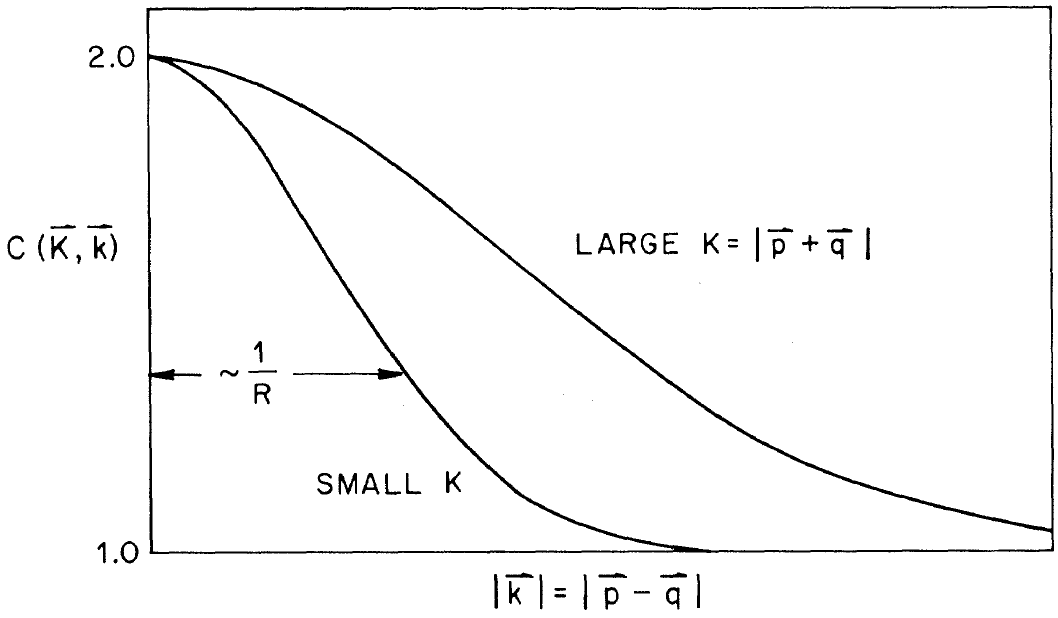
\includegraphics[width=0.75\textwidth]{cf_width_dep}
      \caption{Correlation function width dependence on the total pair momentum. Pion pairs with a large total momentum have a wider correlation (smaller apparent source)~\cite{pratt_pion}.}
      \label{fig:cf_width}
    \end{figure}
    %
    % ========
    \FloatBarrier
    \subsection{Scaling in LCMS}
    % ========
      Hydrodynamic calculations performed in LCMS show that femtoscopic radii in outward, sideward, and longitudinal directions show dependence on transverse mass $m_T~=~\sqrt{k^2_T + m^2}$, where $m$ is a mass of a particle~\cite{akkelin_sinyukov}.
      Moreover, experimental results reveal that this scaling is observed for $R_{LCMS}$ radii as well.
      This dependence can be expressed as follows:
      \begin{empheq}[innerbox=\fbox, right={~,}]{align}
        \label{eq:r_scaling}
        R_i = \alpha m_T^{-\beta}
      \end{empheq}
      where $i$ subscript indicates that this equation applies to $R_{out}$, $R_{side}$ and $R_{long}$ radii.
      The $\beta$ exponent is approximately equal 0.5.
      However, in the case of strong transversal expansion of the emitting source, the decrease of longitudinal interferometry radius can be more quick than $m_T^{-0.5}$.
      Hence, greater values of $\beta >$~0.5 can be expected for longitudinal radii~\cite{akkelin_sinyukov}.
      % \/ do wynikow
      % the scaling behavior shows that hydro produces common collective behavior in both transverse dimensions
    %
    % ========
    \subsection{Scaling in PRF}
    \label{sec:prf_scaling}
    % ========
      In the collisions at the LHC energies, pions are the most abundant particles and their multiplicities are large enough to carry out three-dimensional analysis.
      However, for heavier particles, such as kaons and protons statistical limitations arise.
      Hence, it is often possible to measure only one-dimensional direction-averaged radius $R_{inv}$ for those particles.
      The $R_{inv}$ is then calculated in PRF.
      The transition from LCMS to PRF is a Lorentz boost in the direction of pair transverse momentum with velocity $\beta_T = p_T / m_T$.
      Hence only $R_{out}$ changes:
      \begin{equation}
        R_{out}^* = \gamma_T R_{out}~.
      \end{equation} 
      The Lorentz factor $\gamma_T = m_T / m$ depends on the particle type.
      Therefore, for the lighter particles with the same $m_T$, $\gamma_T$ is much larger resulting in bigger growth of $R_{out}$ and overall radius.
      This transformation to PRF breaks the scaling observed in LCMS radii.

      This increase of radius in the outward direction induces overall source size growth and moreover the source distribution function becomes non-gaussian.
      In this case, the one-dimensional projection of a source function develops long-range tails and is much narrower in comparison to Gaussian distribution.
      This deformation is presented in Fig.~\ref{fig:3dgaussian}.
      The influence of these effects can be expressed with an approximate formula:
      \begin{equation}
        \label{eq:rinv_avg}
        R_{inv} = \sqrt{ \left. \left( {R_{out}}^2\sqrt{\gamma_T} + {R_{side}}^2 + {R_{long}}^2 \right) \middle/ 3 \right. }~.
      \end{equation}
      Because the averaging of the radii is done in quadrature, one would have expected appearance of $\gamma_T^2$ instead of $\sqrt{\gamma_T}$ in this equation.
      However, the Monte-Carlo procedure shows that this is not the case and the actual growth is smaller than the naive expectation.
      Numerical simulations yield that this increase is best described with the $\sqrt{\gamma_T}$ in the Eq.~\ref{eq:rinv_avg}~\cite{galazyn}.

      Assuming that radii in all directions are equal $R_{out} = R_{side} = R_{long}$, Eq.~\ref{eq:rinv_avg} can be reverted using Eq.~\ref{eq:3dradiito1d} to express relationship between LCMS and PRF overall radii~\cite{galazyn}:
      \begin{empheq}[innerbox=\fbox, right=~.]{align}
        R_{LCMS} \approx R_{inv} \times \left[ \left. \left( \sqrt{\gamma_T} + 2 \right) \middle/ 3 \right. \right]^{-1/2}
      \end{empheq}
      This approximate formula allows to restore common scaling of the divided radii not only when they are equal, but also when their differences are small (detailed explanation is given in Section~\ref{sec:source-emission-function}).

      This scaling recovery method in PRF can be used as a tool for the search of hydrodynamic collectivity between pions, kaons and protons in heavy ion collisions with the measurement of one-dimensional radius in PRF.
